\section{Countermeasures}
\label{sec:countermeasures}

Authorization mechanisms like GoodUSB~\cite{tian2015defending} have been
proposed as countermeasures against the BadUSB attack. As mentioned in
Section~\ref{sec:badusb} and Section~\ref{sec:experiment}, GoodUSB relies on
internal display for authorization, which can be bypassed via our \tool. 
%Hence, GoodUSB is indeed a great defense against traditional BadUSB attack but
%no defense at all for our \tool. 
Next, we discuss some effective countermeasures against \tool.

\textbf{External Hardware Authorization.} One possible countermeasure is to
introduce external hardware completing the authorization process. Contrary to
the GoodUSB, USBCheckIn~\cite{usbcheckin} adopts a dedicated hardware between
the host and device. When a device is plugged-in, the authorization will be
conducted on the dedicated hardware instead of the internal display, preventing
the host from being hijacked. Though USBCheckIn is an adequate defense against
\tool, the external hardware brings additional cost and inconvenience,
especially for mobile devices.

\textbf{Distrust-by-Default.} Most security issues of USB protocol are due to
its \textit{trust-by-default} assumption; \tool also relies on this feature to work.
To defend against \tool and other USB-based attacks, we can simply reject all
{unauthorized} device -- applying the \textit{distrust-by-default} policy.  It
is worth mentioning that \textit{distrust-by-default} policy is not the same as
GoodUSB~\cite{tian2015defending}.  \fengwei{the following sentence needs to be
written. I am confused.}\hongyi{Fixed, use more concise sentences} GoodUSB permits limited functionality of untrusted devices while this strict policy forbids all functions of an untrusted device. Though \textit{distrust-by-default} policy effectively
prevents these attacks, it also causes considerable inconvenience for users.

\textbf{Isolated UI Rendering.} During our experiments, we noticed that \tool
is actually unable to redirect out the locking screen keyboard from the iPad
OS. Instead, the keyboard is only available on the internal display. However,
this defense is only enabled on the locking screen keyboard, other keyboards
(e.g., the virtual ones used by the apps) are still vulnerable to our \tool.
This mechanism has inspired us to propose a new defense against our \tool
called \emph{Isolated UI Rendering}. As illustrated in
Figure~\ref{fig:isolated_ui}, we designed two separated UI render layer and corresponding driver, one
is secure the other is insecure. When an application require to render, it can
pass the content along with a tag identifying whether the content is
``sensitive'' or not. If the content is tagged with ``sensitive'', then the OS
will only render it on the secure layer, which only shows the sensitive content
(e.g., a keyboard) on the trusted screen. For the rest of the rendering, it
would render on both trusted and untrusted display (e.g., insensitive
contents).
For example, in Figure~\ref{fig:isolated_ui}, the `password' and `keyboard' are recognized as sensitive while other parts of content are insensitive. Thus, the `password' and `keyboard' are not rendered on untrusted screen as they contains private information.
 \fengwei{we need more text to describe the figure}.

\begin{figure}[t]
	\centering
	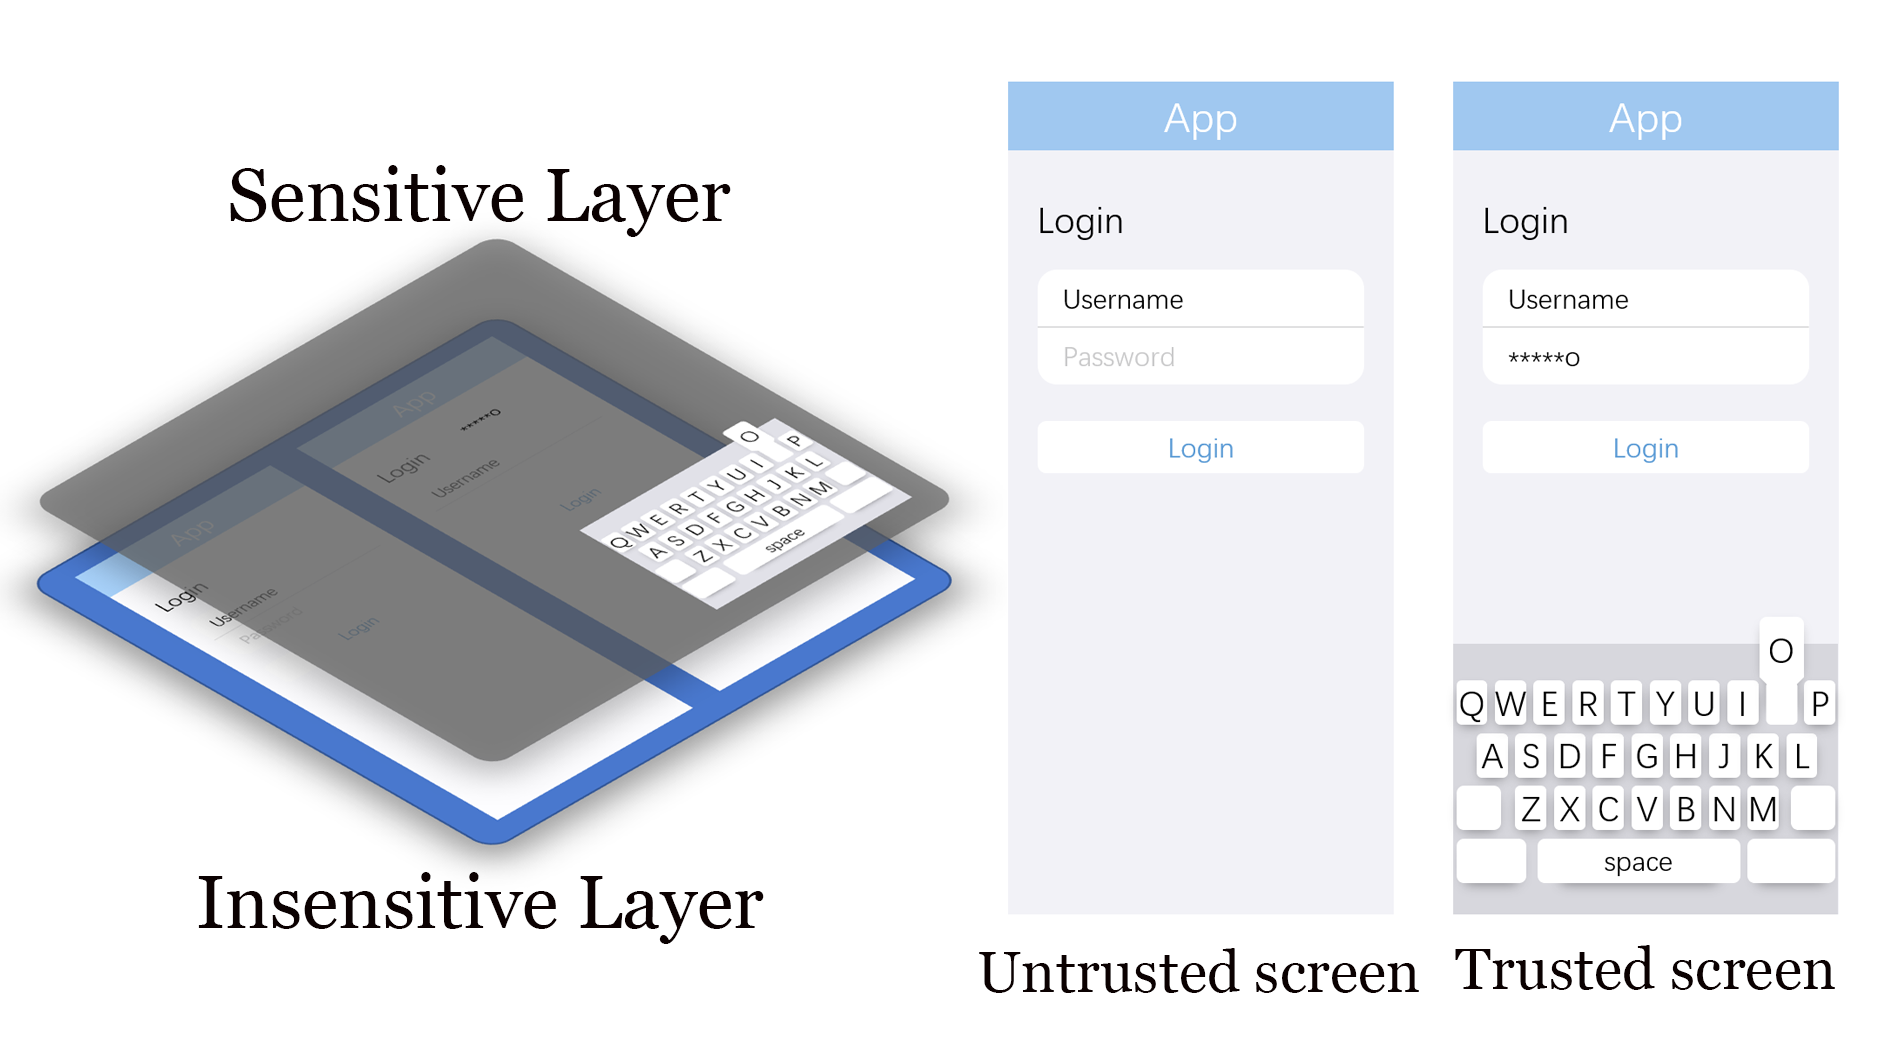
\includegraphics[width=\linewidth]{./Figs/isolated_ui.png}
	\caption{Isolated UI Rendering}%\shuqing{Maybe we can increase the font?}
	\label{fig:isolated_ui}
\end{figure}
\fengwei{what are untrusted and trusted screens? are they internal and external displays?}
\hongyi{Fixed by using the same term and additional description}
